\lhead{\begin{tikzpicture}[remember picture, overlay]
    \node [anchor=100,inner sep=0] (imagenIZQUIERDA) at (current page header area.north){\includegraphics[width=18cm]{img/Encabezado.PNG}};
    \end{tikzpicture}}
    \rhead{Vázquez-Montes}
    \rfoot{\begin{tikzpicture}[remember picture, overlay]
    \node [anchor=140,inner sep=0] (imagenDERECHA) at (current page footer area.south){\includegraphics[width=18cm]{img/Foot.PNG}};
    \end{tikzpicture}}
    %----------------------------------------------------------------------------------------
    \lfoot{ \thepage}
    % \renewcommand{\labelenumi}{\alph{enumi}.)} 
    %----------------------------------------------------------------------------------------
    %----------------------------------------------------------------------------------------
    %	TITLE SECTION
    %----------------------------------------------------------------------------------------
    
    \setlength{\droptitle}{-5\baselineskip} % Move the title up
    \title{\textbf{Estudio de tiempos y movimientos en el ensamble de un circuito electrónico utilizando diferentes métodos para su optimización }} % Article title
    
     \author{ 
         \textsc{Vázquez-Montes,Mitzi Daniela}\\ 
        %  Afiliación:
         \texttt{Instituto Tecnológico de Querétaro} \\ 
         \texttt{Tecnológico Nacional de México} \\ 
         \texttt{Querétaro, México}\\ 
         \texttt{mitzi.vamo25@gmail.com}
     \and 
     \textsc{Ángeles-Hurtado, Luis Alberto}\\ 
    %  Afiliación:
     \texttt{ Instituto Tecnológico de Querétaro } \\ 
     \texttt{ Tecnológico Nacional de México } \\ 
     \texttt{Querétaro, México}\\ 
     \texttt{alb3rt0.ah@gmail.com} 
    }
    
    
    %----------------------------------------------------------------------------------------
    
    % \begin{document}
    
    % Print the title
    \maketitle
    \thispagestyle{fancy}
    
    %----------------------------------------------------------------------------------------
    %	ARTICLE CONTENTS
    %----------------------------------------------------------------------------------------
    
    % \section*{Resumen}
    % \textit{Palabras clave:}
    % El resumen (ancho de página) deberá contener entre 100 y 200 palabras tipo Adobe Devangari 11 puntos.
    
    \begin{abstract}
    \noindent 
    El resumen (ancho de página) deberá contener entre 100 y 200 palabras tipo Adobe Devangari 11 puntos.
    
    \end{abstract}
    % 
    % 
    \textbf{\textit{Palabras clave}}:
    Tiempo,Movimiento, Optimización, Proceso,Ensamble, Productividad.
          
    
    \section{Introducción}
    % \begin{itemize}
    % Define estudio de tiempos y movimientos
    El Estudio de Tiempos y Movimientos es una práctica esencial en la ingeniería industrial que busca mejorar la eficiencia de los procesos combinando el análisis del tiempo de Frederick Winslow Taylor y el estudio de movimientos de Frank y Lillian Gilbreth. \cite{andrade2019estudio} Aplicada en diversas áreas, incluyendo el ensamblaje de circuitos electrónicos, esta técnica utiliza metodologías como el método de tiempos predeterminados, que establece estándares de tiempo para cada actividad basado en una base de datos de tiempos estándar para tareas específicas. Esto facilita la planificación y la optimización continua de la producción industrial \cite{Niebel}.
    Esta técnica es particularmente útil para comprender y mejorar los procesos de fabricación. Por ejemplo, en el ensamblaje de un circuito eléctrico utilizando un Protoboard, permite identificar áreas de mejora y aplicar metodologías adecuadas para optimizar el proceso de ensamblaje. El estudio de tiempos y movimientos abarca el análisis de métodos, materiales, herramientas e instalaciones utilizadas o planificadas para la ejecución de un trabajo, promoviendo una mejora continua en la eficiencia de los procesos industriales.
    % define que es ensamble
    El ensamble consiste en unir, ajustar, montar y encajar piezas, es decir, en la colocación de dos o más piezas para formar un producto final en este caso Un circuito electrónico.
    % define que es circuito electronico
    por su parte, es un conjunto de elementos eléctricos conectados entre sí que generan, transportan y utilizan energía eléctrica para transformarla en otro tipo de energía.
    % define optimización
    En este contexto, definimos la optimización como el proceso de buscar la manera más eficiente de llevar a cabo una actividad específica. En el caso particular de este trabajo, nos enfocamos en optimizar el tiempo empleado en el ensamblaje. \cite{RAE}
    % define el metodo de tiempos predeterminados
    En este proyecto utilizaremos el método de tiempos predeterminados, que establece estándares de tiempo para tareas específicas basándose en una base de datos de tiempos estándar, para eliminar desperdicios de tiempo y aumentar la productividad.
    % Al final se debe hacer alusión al o lo(s) objetivos del proyecto de investigación.
    Para llevar a cabo este proyecto, es fundamental utilizar la optimización y el método de tiempos predeterminados, ya que son herramientas esenciales para alcanzar los objetivos establecidos. En términos generales, estas técnicas contribuyen a una mayor efectividad y éxito, permitiendo definir y lograr los objetivos de manera óptima y eficiente. \cite{Niebel}
    
    
    % \end{itemize}
    % 
    \section{Justificación}
    % \begin{itemize}
    % Cuantos tipos de manufactura existen?
    La manufactura ha experimentado un crecimiento significativo a lo largo de la historia, especialmente a partir del siglo XVIII con la llegada de la primera revolución industrial en Inglaterra.Posteriormente, en los siglos XIX y XX, tuvieron lugar la segunda y la tercera revolución industrial, impulsando aún más la evolución de la manufactura hacia un proceso altamente sofisticado y tecnológico. En la actualidad, la manufactura abarca una amplia variedad de enfoques que continúan evolucionando con el tiempo. Podemos identificar al menos ocho tipos distintos de manufactura que se aplican en diversas industrias. Estos enfoques reflejan la adaptabilidad y la innovación constante dentro del campo de la producción industrial. \cite{Revoluciónindustrial}
    % Cuantas empresas de manufactura existen en Mundo?
    Se estima que en el mundo existen millones de empresas de manufactura, que abarcan desde pequeñas y medianas empresas,hasta grandes corporaciones multinacionales. Sin embargo, no hay un número exacto que describa la cantidad de estas empresas, ya que esta cifra está en constante cambio debido a diversos factores, como la creación constante de nuevas empresas y la evolución del panorama empresarial.
    % Cuantas empresas de manufactura existen en México?
    Según datos del INEGI, en 2018 se registraron 579,828 establecimientos dedicados a las manufacturas en México. Estas actividades abarcan una amplia variedad de sectores, como la producción de alimentos y bebidas, la elaboración de maquinaria y productos textiles, entre otros. \cite{Cuéntamedemexico}
    % Cuantas empresas de manufactura existen en Querétaro?
    Además, se observa un aumento continuo en el número de establecimientos manufactureros. Un ejemplo de ello es el estado de Querétaro, donde se contabilizan 7,649 establecimientos dedicados a la manufactura en censos económicos del 2019.
    % \end{itemize}
    % 
    % 
    \section{Descripción del problema}
    Los estudiantes del Instituto Tecnológico de Querétaro desempeñan un papel vital en el impulso del crecimiento económico y desarrollo tecnológico de México. La inversión en educación superior son papeles fundamentales para construir una economía sólida y así poder garantizar un futuro próspero para ellos.
    Los estudiantes del Instituto Tecnológico de Querétaro deben adquirir habilidades en tendencias tecnológicas para mantenerse competitivos a nivel mundial.
    Los estudiantes deberían contar con el tiempo adecuado para este tipo de prácticas, para así adquirir habilidades esenciales y disponer de los recursos educativos. 
    % 
    % 
    \section{Fundamentación teórica}
    
    %Es la parte medular y de mayor discusión, deberá ser la fundamentación de la hipótesis, por tanto se deberá señalar claramente la razón de la suposición y fundamentación de la misma. Únicamente referencias científicas.
    %\begin{itemize}
       % \item Se debe de retomar el tema que se planteo en la introducción, pero ahora profundizando para clarificar la incógnita científica y se pueda plantear la hipótesis.
      %  \item Se debe de retomar la descripción del problema, pero ahora a profundidad del (los) objeto(s) de estudio. 
      %  \item Se debe de profundizar en las metodologías que se ha usado para el estudio del tema.
      %  \item Referencias solo de artículos y libros científicos.
    %\end{itemize}
    
    % Cuales son las revoluciones industriales que ha vivido la humanidad?
    Durante los últimos dos siglos, el mundo ha sido testigo de tres revoluciones industriales y tecnológicas que han transformado profundamente a la sociedad. Cada una de estas revoluciones, se han modificado las fuentes de energía, sectores industriales, ubicación geográfica y los medios de comunicación utilizados para el transporte de bienes, personas e información.
    La primera tuvo lugar en el siglo XVIII en Inglaterra, seguida por la segunda y tercera revolución industrial en los siglos XIX y XX respectivamente.
    
    % A lo largo de la historia del hombre las técnicas manuales para elaborar herramientas y mejorar la caza y la calidad de vida fueron fundamentales para la supervivencia.
    % La revolución industrial han cambiado las fuentes de energía básicas y los medios de comunicación para desplazar mercancías, personas e información.
    % 
    % 
    \section{Hipótesis}
    Desarrollar un proyecto integrador en Estudio del Trabajo II potenciará las habilidades del estudiante al máximo. Este proyecto se enfocará en determinar el tiempo estándar en el ensamblaje de circuitos electrónicos, abordando todos los temas vistos en clase. Para enriquecerlo, se analizará el impacto de los componentes en el tiempo de ensamblaje y se implementarán herramientas de simulación como SOLIDWORKS, este software facilitará al operador seguir el manual de ensamblaje de una manera más eficiente.
    Este enfoque integral preparará al estudiante para desafíos reales en el campo del trabajo y la producción electrónica.
    % 
    % 
    \section{Objetivo}
    El estudiante deberá adquirir los conocimientos básicos para la elaboración de este proyecto. Además pondrá en práctica sus habilidades para determinar el porcentaje de tiempo productivo, establecer tolerancias y calcular el tiempo estándar. Todo esto se deberá realizar en un periodo de seis meses, de Enero a Junio del presente año, y será documentado en el proyecto integrador.
    \begin{itemize}
        \item Diseña, mejora e integra sistemas productivos de bienes y servicios aplicando tecnologías para su optimización.
        \item Diseña, implementa mejoras de trabajo para elevar la productividad.
    \end{itemize}
    
    \subsection{Objetivos específicos }
    \begin{itemize}
        \item Desarrollar una guía de emergencia para analizar la instalación en la que se llevo acabo la experimentación.
        \item Analizar los métodos, materiales, herramientas e instalación utilizada o que se ha de utilizar en la ejecución del ensamble de un circuito electrónico.
        \item Se establecerá la forma más económica de realizar el trabajo.
        \item Normalizar los métodos, materiales, herramientas e instalaciones.
        \item Determinar exactamente el tiempo necesario para que una persona competente realice el trabajo con una marcha normal.
    \end{itemize}
    
    \section{Metodología}
    El trabajo de investigación se realizó mediante observación y análisis estadístico en el Instituto Tecnológico de Querétaro (ITQ) durante el periodo de febrero a mayo de 2024. El estudio se centró en el ensamblaje de una tarjeta electrónica utilizando un software de diseño asistido por computadora. En la primera etapa de la experimentación, se tomaron dos muestras continuas con una cámara de vídeo y finalmente se implementaron diversas metodologías para obtener el tiempo de ciclo y el tiempo estándar. Esta recolección de datos se realizó en el edificio C, salón C07 del Tecnológico Nacional de México Campus Querétaro. 
    Para llevar a cabo el circuito electrónico se llevaron a cabo los siguientes pasos: Preparación de materiales: Verificar la disponibilidad y buen estado de todos los componentes necesarios. Véase la figura \ref{fig:enter-label1} Preparación del espacio de trabajo: Asegurar un espacio limpio, bien iluminado y equipado con herramientas específicas como la almohadilla para soldar y multicontacto. Véase la figura \ref{fig:enter-label2} Ensamble de componentes: Seguir el Manual de ensamblaje del ESP32-C6 para la correcta instalación de los componentes. Véase la figura \ref{fig:enter-label3}
    Las imágenes explican detalladamente varios aspectos de los procedimientos, Véase la figura \ref{fig:enter-label4} está muestra el procedimiento utilizado para comprobar la hipótesis, en la figura \ref{fig:enter-label5} se muestra la cadena de medida utilizada y finalmente en la figura \ref{fig:enter-label6} detalla las interacciónes de flujos de datos, con ello se muestran los datos resumidos para asi determinar la forma más económica de hacer el trabajo, en este caso el ensamble.
    
    \begin{figure}[H]
        \centering
        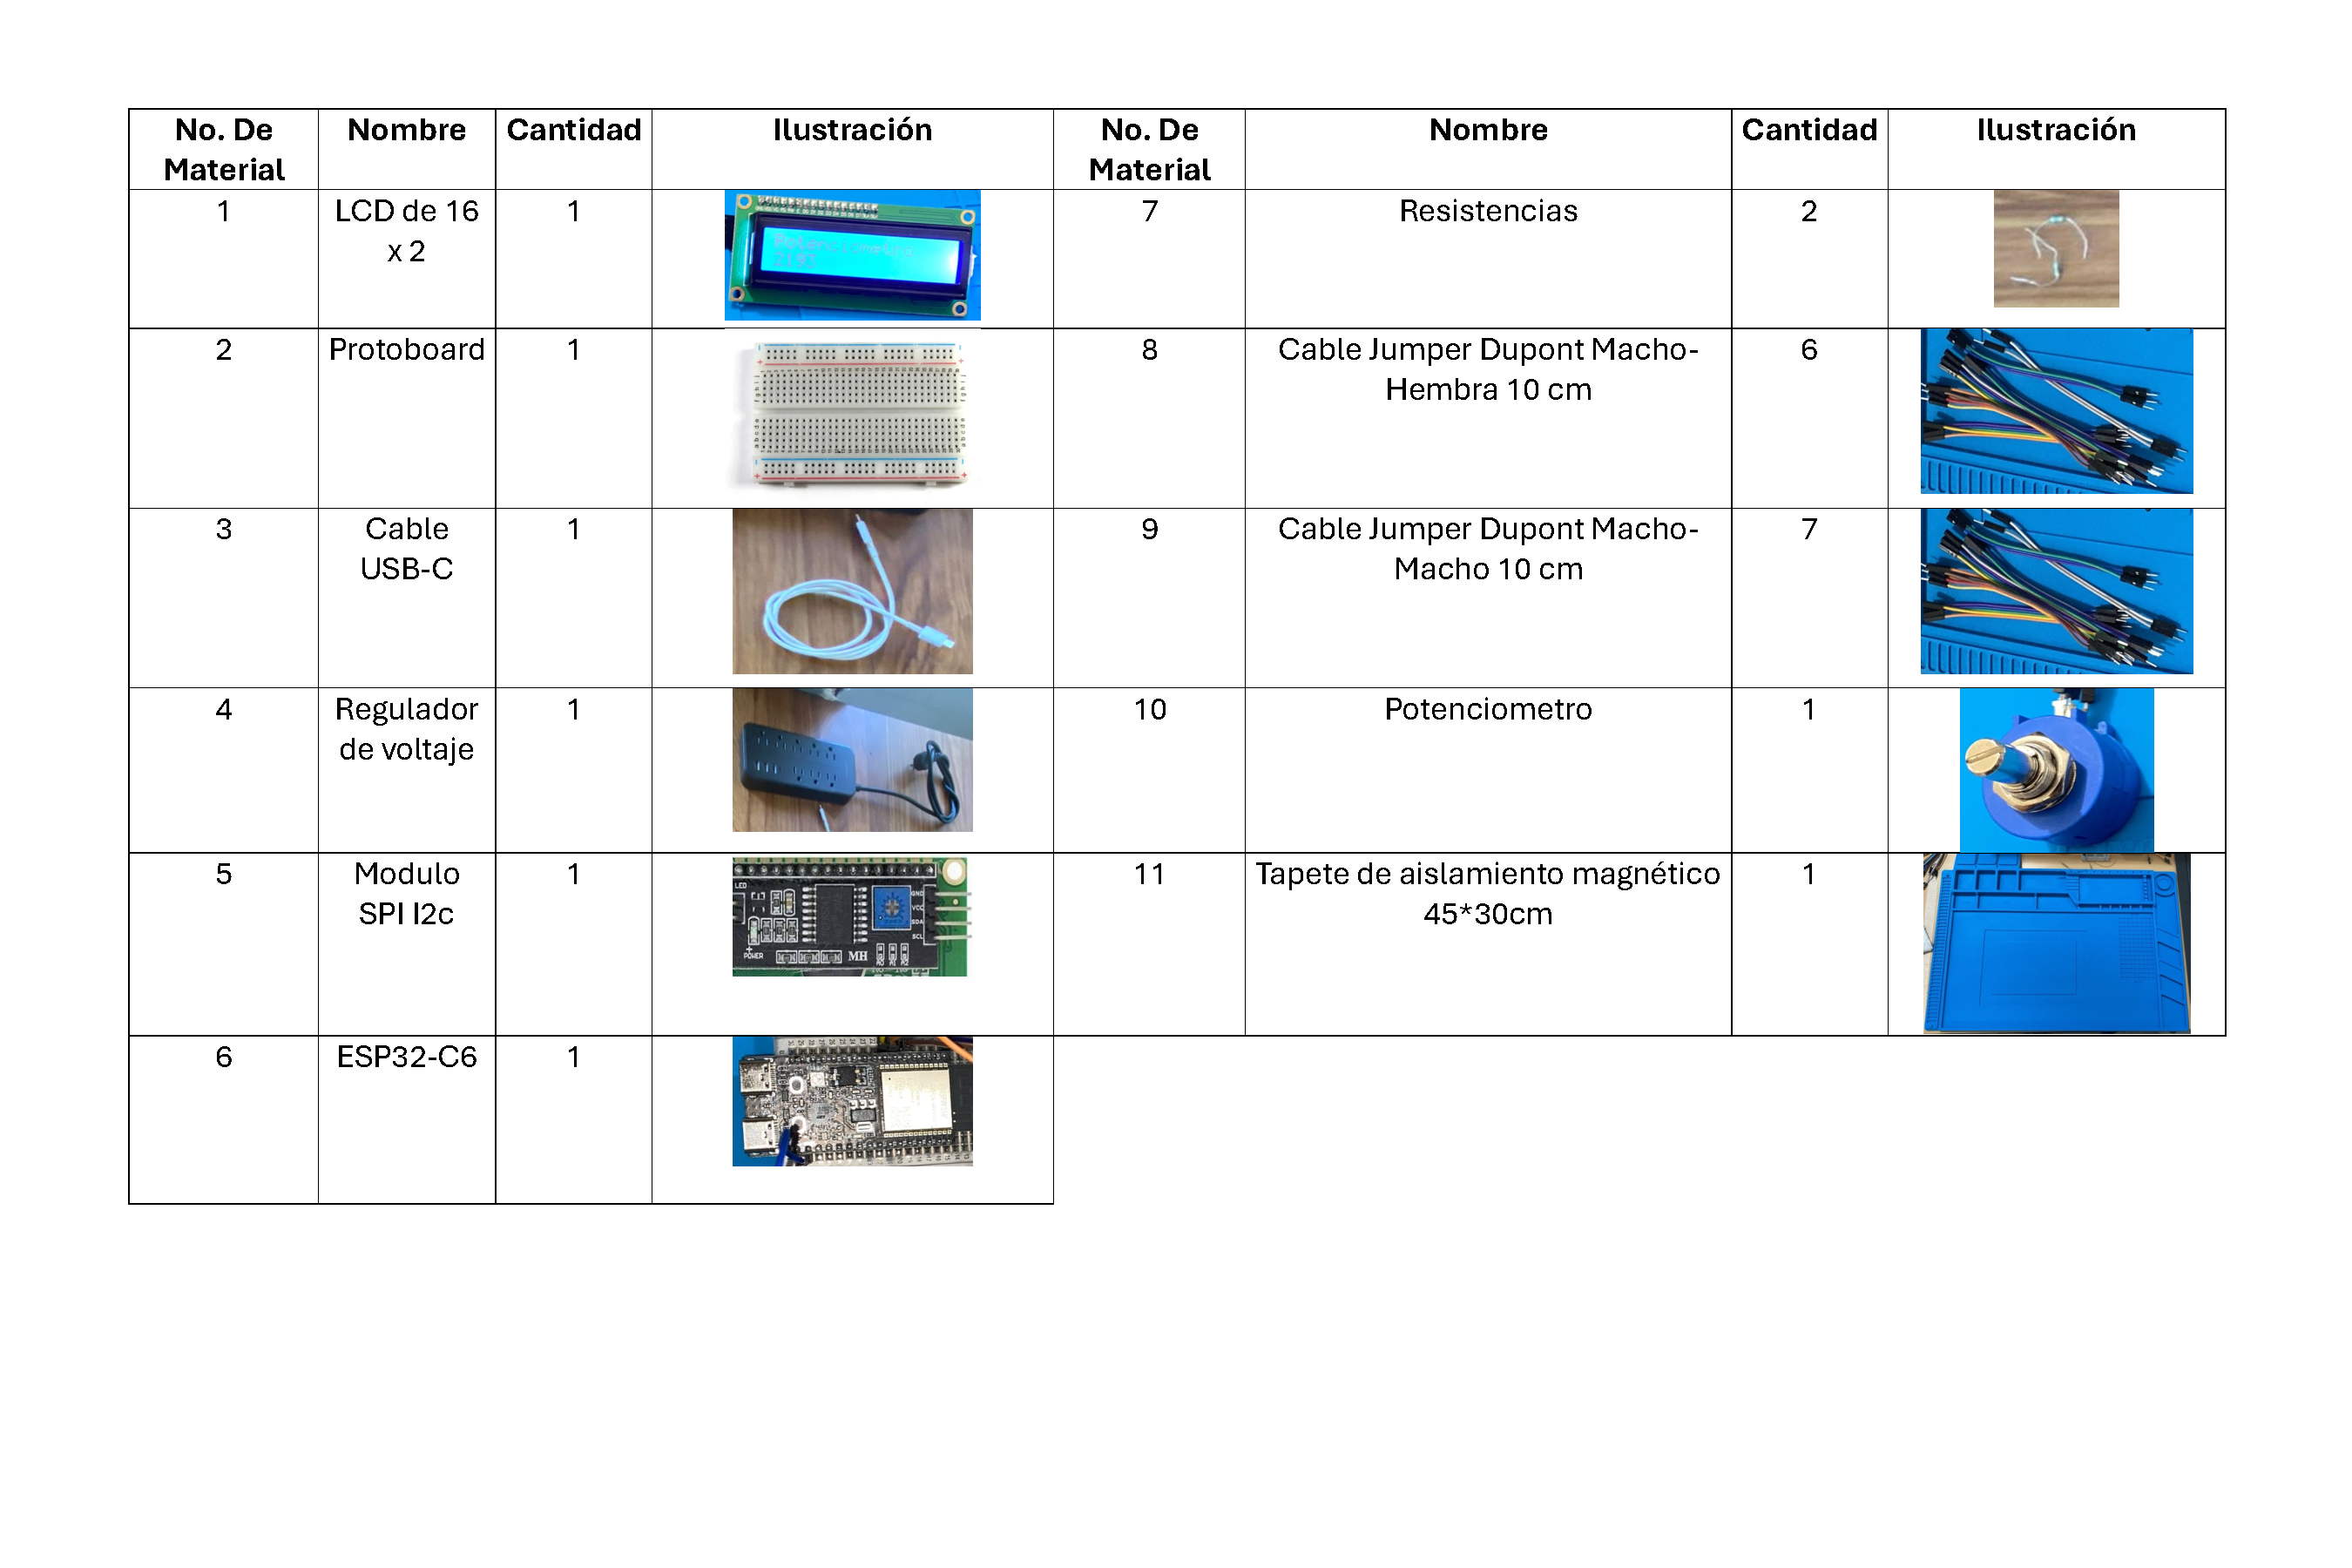
\includegraphics[trim = {1mm 1mm 1mm 1mm},clip,scale=0.2]{34/img/listaDeMateriales.png}
        \caption{Lista de materiales}
        \label{fig:enter-label1}
    \end{figure}
    \begin{figure}[H]
        \centering
        \includegraphics[trim = {1mm 1mm 1mm 1mm},clip,scale=0.2]{34/img/bosquejo.png}
        \caption{Bosquejo}
        \label{fig:enter-label2}
    \end{figure}
    \begin{figure}[H]
        \centering
        \includegraphics[trim = {1mm 1mm 1mm 1mm},clip,scale=0.2]{34/img/pasosEnsamble.png}
        \caption{Pasos ensamble}
        \label{fig:enter-label3}
    \end{figure}
    \begin{figure}[H]
        \centering
        \includegraphics[trim = {1mm 1mm 1mm 1mm},clip,scale=0.2]{34/img/diagramaMetodología.png}
        \caption{Diagrama de metodología}
        \label{fig:enter-label4}
    \end{figure}
    
    \begin{figure}[H]
        \centering
        \includegraphics[trim = {1mm 1mm 1mm 1mm},clip,scale=0.2]{34/img/cadenaDeMedida.png}
        \caption{Cadena de medida}
        \label{fig:enter-label5}
    \end{figure}
    
    \begin{figure}[H]
        \centering
        \includegraphics[trim = {1mm 1mm 1mm 1mm},clip,scale=0.2]{34/img/diagramaEntradaSalida.png}
        \caption{Diagrama de entradas y salidas}
        \label{fig:enter-label6}
    \end{figure}
    
    
    
    % 
    % \begin{figure}[H]
    %     \centering
    %     \includegraphics[trim = {30mm 250mm 90mm 20mm},clip,scale=0.5]{6/Img/lcd-16x2.pdf}
    %     \caption{Esquema LCD de 16x2}
    %     \label{fig:lcd-16x2}
    % \end{figure}
    % 
    % 
    \subsection{Desarrollo de la guía de plan de Emergencia}
    El plan de emergencia es crucial para la universidad, ya que sin él, enfrentaríamos serios problemas en situaciones de crisis. Es fundamental conocerlo en detalle, dado que los riesgos son dinámicos y todos estamos expuestos a ellos. Familiarizarnos con este plan garantiza que estemos preparados para actuar de manera efectiva y segura ante cualquier eventualidad que se pueda presentar.Esta guía se elaboró mediante la recopilación y análisis de datos sobre los procesos de emergencia de la institución. Se clasificaron los riesgos internos y externos, asignándoles una probabilidad de ocurrencia. Se diseñó un programa de prevención y auxilio, junto con un plan de acción y la identificación de capacidades. Se evaluó la ubicación de recursos, como la señalización, los extintores de emergencia y los botiquines. Se identificaron los riesgos externos y los puntos de reunión. Además, se formó una brigada de evacuación y se estableció un directorio telefónico de emergencia.
    % 
    \subsection{Análisis de los métodos, materiales, herramientas e instalación utilizada en la ejecución del ensamble de un circuito electrónico}
    
    \subsubsection{Planeación}
    Para este proyecto, se planea identificar la forma más económica de realizar el trabajo. Nos enfocaremos en identificar áreas de mejora, reducir el tiempo de ciclo y eliminar movimientos innecesarios. Para ello, se recolectarán datos mediante una cámara que grabará un vídeo continuo, permitiendo determinar el tiempo. 
    Para llevar a cabo lo mencionado anteriormente, se planea utilizar una serie de materiales que nos ayudarán a realizar el ensamblaje de manera óptima. El profesor nos ha proporcionado los materiales a utilizar, véase la lista de materiales en la figura \ref{fig:enter-label1} en dónde se muestra el modelo de la pieza así como también su costo por unidad.
    Cada material debe ser meticulosamente evaluado mediante mediciones, tacto, olfato y cualquier otro método necesario para obtener una comprensión completa de sus características. Estos datos se plasman en un programa asistido por computadora, en este caso, se utilizó SolidWorks versión 2019, para especificar las dimensiones de cada uno de los materiales de manera detallada y precisa. A continuación se muestran de forma más detalladas las piezas a utilizar.
    
    \begin{figure}[H]
        \centering
        \includegraphics[scale=0.3]{34/img/reguladorVoltaje.png}
        \caption{Regulador de voltaje Componente que mantiene
    una salida de voltaje constante independientemente
    de las variaciones en la entrada o en la
    carga.}
        \label{fig:reguladorVoltaje}
    \end{figure}
    
    \begin{figure}[H]
        \centering
        \includegraphics[scale=0.3]{34/img/protoboard.png}
        \caption{Protoboard versiónn de 300 puntos de conexión, organizados en filas y columnas con carriles de alimentación en los bordes.}
        \label{fig:protoboard}
    \end{figure}
    
    \begin{figure}[H]
        \centering
        \includegraphics[scale=0.3]{34/img/esp32C6.png}
        \caption{El ESP32-C6-WROOM-1 es un dispositivo utilizado en el desarrollo de aplicaciones para el Internet de las Cosas (IoT), controladores embebidos y proyectos que necesitan conectividad inalámbrica.}
        \label{fig:esp32C6}
    \end{figure}
    
    \begin{figure}[H]
        \centering
        \includegraphics[scale=0.3]{34/img/resistencia.png}
        \caption{Resistencias de 330 Ohms Su tarea es regular la corriente y distribuir los voltajes en los circuitos electrónicos.}
        \label{fig:resistencia1}
    \end{figure}
    
    \begin{figure}[H]
        \centering
        \includegraphics[scale=0.3]{34/img/dupontMachoHembra.png}
        \caption{Dupont-10 Hembra-Macho Conjunto de cables con un conector hembra en un extremo y un conector macho en el otro, de 10 cm de longitud.}
        \label{fig:resistencia2}
    \end{figure}
    
    \begin{figure}[H]
        \centering
        \includegraphics[scale=0.3]{34/img/dupontMachoMacho.png}
        \caption{Cables Dupont-10 Macho-macho Conjunto de cables con conectores macho en ambos extremos, de 10 cm de longitud.}
        \label{fig:resistencia}
    \end{figure}
    
    \begin{figure}[H]
        \centering
        \includegraphics[scale=0.3]{34/img/cableUsbC.png}
        \caption{Cable USB-C es un cable de conexión con conector USB-C en un extremo.}
        \label{fig:cableUsbC}
    \end{figure}
    
    
    \begin{figure}[H]
        \centering
        \includegraphics[scale=0.3]{34/img/lcd16x2.png}
        \caption{LCD Display 16x2 Es una pantalla de cristal líquido con 16 columnas y 2 filas de caracteres. Generalmente con retro iluminación LED.}
        \label{lcd16x2}
    \end{figure}
    
    \begin{figure}[H]
        \centering
        \includegraphics[scale=0.3]{34/img/potenciómetro1KOhm.png}
        \caption{Potenciómetro 3540S-1-501L Este es un potenciómetro de precisión con un valor de resistencia
    de 500 ohmios y un diseño robusto.}
        \label{potenciómetro1KOhm}
    \end{figure}
    
    \begin{figure}[H]
        \centering
        \includegraphics[scale=0.3]{34/img/móduloSpi.png}
        \caption{Módulo SPI 12C Es un adaptador o convertidor
    que permite la comunicación entre dispositivos usando los protocolos SPI (Serial Peripheral Interface) e I2C (Inter-Integrated Circuit).}
        \label{móduloSpi}
    \end{figure}
    
    Se elaboró un manual detallado para el ensamblaje, seguido por la grabación de dos muestras en vídeo del operador trabajando en diferentes días y condiciones. Estas muestras se utilizarán para determinar el tiempo estándar de trabajo y se implementarán mejoras, incluida la metodología de las 5 S, con el objetivo de optimizar los procesos. Se realizará también un análisis de costos para identificar la manera más económica de realizar el trabajo. La pieza clave indispensable para el ensamblaje es la programación de una ESP-32, ya que sin ella no se podría completar el proceso. Con estos materiales, estaremos listos para empezar a realizar las muestras utilizando una cámara. La primera muestra se llevará a cabo el 25 de abril del presente año y la segunda muestra se realizará al menos una semana después. Este intervalo de tiempo permitirá capturar variaciones potenciales en el proceso de ensamblaje.
    % 
    \subsubsection{5's}
    El mantenimiento de un espacio limpio y ordenado no solo responde a criterios estéticos, sino que también es un reflejo directo de la calidad de nuestro trabajo. Por esta razón, en el proceso de ensamblaje, resulta crucial la implementación de las 5S. \cite{PgSantos}
    Con estas prácticas, queremos que el operador adopte estas acciones como parte natural de su trabajo diario, no como algo que hace ocasionalmente. Queremos que se convierta en un hábito arraigado en todo el equipo, algo que hagan de forma automática y consistente. Esta mentalidad se alinea con el principio de "Shitsuke", el cual implica la disciplina y el compromiso con la mejora continua. Durante el proceso, la estación de trabajo del operador se mantuvo impecable de principio a fin, gracias a la implementación de la "Seiso" (limpieza), asegurando así condiciones óptimas para llevar a cabo las tareas de manera eficiente. Además, la siguiente imagen de referencia    muestra claramente la meticulosa organización del operador en cuanto a herramientas y materiales,  demostrando la aplicación de la "Seiton" (orden), lo que refuerza la importancia de mantener un entorno limpio y ordenado para garantizar la eficiencia y calidad en todas las operaciones. \cite{manzano2016lean}Veáse la figura \ref{fig:5s}
    \begin{figure}[H]
         \centering
         \includegraphics[scale=0.4]{34/img/aplicandoLas5S.png}
         \caption{Ejemplo en dónde se observa al operador aplicando las 5s}
         \label{fig:5s}
     \end{figure}
    %
    % 
    \subsubsection{Desarrollo del sistema de tiempos predeterminado}
    El sistema de tiempos predeterminados (STP) es ideal para este proyecto porque permite dividir las tareas en detalle y asignar tiempos precisos a cada una. Esto facilita la planificación, optimización de recursos y mejora de la productividad, asegurando procesos eficientes. Para desarrollar los STP, seguimos pasos basados en los Therbligs, aplicados por un analista capacitado, lo que permite predecir con precisión los tiempos necesarios y realizar un análisis de métodos. Estos pasos se dividen en tres fases principales:
    
    1- Dividir el trabajo en elementos: Todos los movimientos del operario se dividen en 10 categorías: alcanzar, mover, girar, aplicar presión, asir, colocar, soltar, separar, movimientos del cuerpo y movimientos de los ojos. \cite{ronquillo2021analisis}
    \begin{figure}[H]
            \centering
            \includegraphics[trim = {1mm 1mm 1mm 26mm},clip,scale=0.3]{34/img/tablaAlcanzarR.pdf}
            \caption{Tabla 1 Alcanzar R}
            \label{fig:tablaAlcanzarR}
        \end{figure}
    
    \begin{figure}[H]
            \centering
            \includegraphics[trim = {1mm 1mm 1mm 26mm},clip,scale=0.3]{34/img/tablaMoverM.pdf}
            \caption{Tabla 2 Mover M}
            \label{fig:tablaMoverM}
        \end{figure}
    
        \begin{figure}[H]
            \centering
            \includegraphics[trim = {1mm 1mm 1mm 26mm},clip,scale=0.3]{34/img/tablaGirar.pdf}
            \caption{Tabla 3 Girar y aplicar presión T Y AP}
            \label{fig:tablaGirar}
        \end{figure}
    
        \begin{figure}[H]
            \centering
            \includegraphics[trim = {1mm 95mm 200mm 26mm},clip,scale=0.4]{34/img/tablaSoltar.pdf}
            \caption{Tabla 6 Soltar RL}
            \label{fig:tablaSoltar}
        \end{figure}
        
        
    
    2- Asignar valores de tiempo a cada elemento: Se utilizan las Unidades de Medida de Tiempo (TMU). Por ejemplo, la acción de "alcanzar" se subdivide en 5 casos, y la acción de "mover" se subdivide en 3 casos, considerando la relación con el peso del objeto o su resistencia al movimiento.
    
    3- Sumar los tiempos de todos los elementos: Después de clasificar todos los movimientos y asignarles un valor, se suman los tiempos de todos los movimientos para obtener el tiempo total necesario para completar la tarea.
    
    Este proceso permite predecir con precisión el tiempo necesario para realizar un trabajo y facilita la optimización de los recursos y la mejora de la productividad.
    
    
    
    
    
    
    
    % 
    \subsubsection{Desarrollo del muestreo del trabajo}
    
    
    % 
    \subsubsection{Corrección por balanceo de procesos}
    El propósito principal de este proyecto es minimizar el tiempo de ciclo y maximizar la eficiencia y productividad del sistema de producción en este caso del ensamble de la ESP-32. Gracias al operador podemos evitar cuellos de botella y desequilibrios en la carga de trabajo entre las estaciones, para así garantizar un flujo constante y óptimo de producción. Con esta metodología buscamos determinar el número adecuado de operadores que necesitaremos y con ellos poder distribuir las tareas uniformemente entre las estaciones de trabajo, ajustándolas según el tiempo estándar y el ritmo de producción necesario. Además, mediante la corrección por balanceo de procesos, se busca optimizar la distribución del trabajo para minimizar el tiempo ciclo y maximizar la eficiencia en la producción.
    % 
    \subsubsection{Datos estándar continuos y discretos}
    Cuando se trata de datos cuantitativos, es importante distinguir entre variables discretas y continuas. Una variable es discreta si solo puede tomar valores específicos y distintos, sin tener ningún valor entre dos consecutivos. Por otro lado, una variable continua puede asumir cualquier valor dentro de un intervalo dado. Al comprender esta distinción, podemos clasificar de manera precisa los tipos de datos que estamos manejando y aplicar los métodos estadísticos adecuados para su análisis. \cite{Datoscontinuosydiscretos}
    % 
    \subsection{Diseño de la forma más económica de realizar el trabajo}
    En este proyecto integrador, nuestro objetivo principal es diseñar la forma más económica de realizar el trabajo. Para ello, llevaremos a cabo un análisis exhaustivo de los procesos y determinaremos el tiempo ciclo estándar del ensamblaje. Utilizaremos el muestreo de trabajo como una herramienta clave para lograrlo, permitiéndonos evaluar y optimizar los tiempos. Esto nos ayudará a reducir los costos asociados y a mejorar la eficiencia, proporcionando datos precisos y continuos para el estudio y ajuste de los tiempos de trabajo. A través de esta metodología, aseguramos una producción equilibrada y económicamente eficiente.
    % 
    % 
    \subsection{Normalización de los métodos, materiales, herramientas e instalaciones}
    % 
    % 
    \subsection{Determinación del tiempo estándar para que una persona competente realice el trabajo con marcha normal}
    La fórmula de la media de la variable aleatoria discreta x es:
    
    \begin{equation}
        \mu_x=\dfrac{b+a}{2}
    \end{equation}
    
    La fórmula de la desviación estándar de X es:
    
    \begin{equation}
    \sigma_x=\sqrt{\dfrac{(b-a+1)^2-1}{(12}}
    \end{equation}
    
    %\subsection{Acrónimos y Abreviaciones}
    
    %Los acrónimos y abreviaciones deberán ser definidos únicamente la primera vez que aparecen en el texto, esto para que el lector entienda lo que significan.
    
    %\subsection{Ecuaciones}
    
    %Las ecuaciones son una excepción a las especificaciones prescritas de esta plantilla. 
    %Deberá determinar si su ecuación debe escribirse o no utilizando la fuente Adobe Devangari. 
    %Para crear ecuaciones multinivel, puede ser necesario tratar la ecuación como un gráfico e insertarla en el texto después de aplicar el estilo de la platilla.
    %Las ecuaciones serán enumeradas de manera consecutiva, y el número de ecuación, entre paréntesis, se colocan al ras de la derecha, utilizando una tabulación derecha. 
    
    %\begin{equation}
    %    \label{eq1}
     %   x + y = z 
    %\end{equation}
    
    %Es importante asegurarse de que los símbolos de la ecuación sean definidos antes o inmediatamente después de la ecuación. Utilice “(1)”, en vez de “Eq. 1” al enumerar las ecuaciones, excepto al principio de una oración: “La ecuación (\ref{eq1}) es…”
    
    \section{Resultados y discusión}
    
     \subsection{Desarrollo de la guía de plan de Emergencia}
    Implementación de estrategias para garantizar seguridad en el Instituto Tecnológico de Querétaro mediante procedimientos de emergencia antes, durante y después de situaciones de riesgo, con énfasis en la capacitación anual del personal para tomar decisiones adecuadas en salvaguarda de la integridad física y de las instalaciones. Los datos generales de la institución se muestran en la figura \ref{fig:enter-label7} así como la fachada de referencia se muestra en la figura \ref{fig:enter-label8}
    \begin{itemize}
        \item Tecnológico Nacional de México campus Querétaro, Instituto Tecnológico de Querétaro (ITQ)
    \begin{figure}[H]
        \centering
        \includegraphics[scale=0.4]{34/img/direcciónItq.png}
        \caption{Dirección del: Tecnológico Nacional de México Campus Querétaro Av Tecnológico S/N, Centro Histórico, Centro, 76000 Santiago de Querétaro, Qro. 442 227 44 00 Ext. 4423}
        \label{fig:enter-label7}
    \end{figure}
    \begin{figure}[H]
        \centering
        \includegraphics[scale=0.3]{34/img/itq.png}
        \caption{Fachada del instituto}
        \label{fig:enter-label8}
    \end{figure}
    Somos una Institución de Educación Superior y Posgrado que forma profesionales mediante un modelo educativo integral de calidad, que garantiza una formación técnica humanística, con capacidad para investigar y aplicar tecnología con impacto en el desarrollo de la sociedad. Nuestro lema es Lema "Tlalticpac Toquichtin Tiez", es un proverbio Náhuatl que se traduce como “La Tierra será como sean los hombres” 
    
    \item Dirección a cargo de Ramón Soto Arriola	\textbf{Correo:} dir@queretaro.tecnm.mx	\textbf{Extensión:} 4429
    \item \textbf{Cantidad de trabajadores:242}
    \item \textbf{superficie 78,271.42 m2}
    \end{itemize}
    %
    \subsubsection{Identificación del riesgo}
    Es importante contar dentro del inmueble con planes de acción para casos de riesgos, estos nos ayudarán al manejo y control de los riesgos que puedan ocurrir, es de suma importancia mantener este compromiso interno, así como la continua retroalimentación del mismo, el objetivo de dicho plan, serpa el ayudarnos a evaluar la gravedad del riesgo de un acontecimiento y de esta manera determinar la mejor acción a seguir.
    
    \begin{figure}[H]
        \centering
        \includegraphics[scale=0.15]{34/img/diagrama.png}
        \caption{Diagrama para la identificación de riesgos y acciones}
        % \label{fig:enter-label9}
    \end{figure}
    
    \subsubsection{ Riesgos Internos}
    El riesgo se define como la contingencia o proximidad de un daño.\cite{RAE} Es decir, se refiere a la posibilidad de que ocurra un evento adverso que pueda causar perjuicio, pérdida o daño a una persona, entidad o bienes. El riesgo implica una incertidumbre respecto al futuro, donde se evalúan tanto la probabilidad de que ocurra un evento adverso como las consecuencias que dicho evento podría tener en el funcionamiento, la seguridad y el bienestar de la comunidad universitaria.
    Se deberán identificar los riesgos a los que esta expuesto el Instituto Tecnológico de Querétaro de manera interna, así como también la identificación de los riesgos a los que se encuentra expuesta la zona donde se ubica y que pueden incidir en el mismo.
    
    \begin{table}[h]
        \centering
        \caption{Riesgos con diferentes niveles y colores para distinguir la gravedad y acciones}
        \begin{tabular}{c c c}
        \hline
        \multicolumn{3}{c}{\textbf{Riesgos}}\\
        \hline
             Alto& 0.99 - 0.18 & Rojo  \\
        \hline
             Medio& 0.17 - 0.05 & Amarillo  \\
        \hline
             Bajo& 0.04 - 0.01 & Verde \\
        \hline     
        \end{tabular}
        \label{tab:riego}
    \end{table}
    
    \begin{figure}[H]
        \centering
        \includegraphics[trim = {1mm 120mm 1mm 1mm},clip,scale=0.45]{34/img/riesgoInternoActividadesComunes.pdf}
        \caption{Descripción de los riesgos internos al realizar actividades comunes dentro de la institución}
        \label{fig:enter-label10}
    \end{figure}
     
    \subsubsection{Riesgos externos}
    
     \begin{table}[H]
         \centering
    \caption{Descripción de los riesgos externos}
        \begin{tabular}{|p{4em}|p{6em}|c|p{6em}|}
             \hline
             \textbf{Riesgo}& \textbf{Probabilidad}& \textbf{Impacto}& \textbf{Acciones preventivas}\\
             \hline
             Robo & 0.04& Muy bajo& Instalar cámaras, alarmas e iluminación.\\
             \hline
              Choque en la avenida& 0.17 & Medio&Poner conos de señalamiento.\\
              \hline
              Desastre natural& 0.17& Medio& Sistemas de drenaje eficientes, mantenimiento y limpieza constante.\\
              \hline
             Incendios& 0.99& Alto& Colocar extintores,mangueras y crear un plan de emergencia para incendios\\      
              \hline
    
         \end{tabular}
         \label{tab:RiesgosExternos}
    \end{table}
    % 
    \subsubsection{Programa de actividades de prevención y auxilio}
    
    %Declaramos las diferentes acciones de lo que se piensa hacer cuando ocurra un riesgo interno u externo. 
    %Las actividades de preparación y disposición que se hace anticipadamente en el ITQ para evitar riesgos.
    % 
    % 
    \subsubsection{Plan de acción}
    Ante posibles interrupciones en las operaciones del Instituto Tecnológico de Querétaro, es crucial contar con procedimientos ágiles que garanticen su continuidad. Se requiere la participación de toda la comunidad tecnológica en un plan de acción que asegure la continuidad de procesos y servicios críticos. La colaboración de todos es esencial para identificar riesgos, implementar medidas preventivas y establecer protocolos de actuación claros. Al priorizar la continuidad operativa, se protege el funcionamiento y la seguridad de la comunidad del Instituto.
    
    \begin{figure}[H]
        \centering
        \includegraphics[trim = {1mm 120mm 1mm 10mm},clip,scale=0.45]{34/img/riesgoInterno.pdf}
        \caption{Descripción de acciones anticipadas de riesgos internos}
        \label{fig:enter-label11}
    \end{figure}
    
    \begin{figure}[H]
        \centering
        \includegraphics[trim = {1mm 129mm 1mm 1mm},clip,scale=0.45]{34/img/riesgoExterno.pdf}
        \caption{Descripción de acciones anticipadas de riesgos externos}
        \label{fig:enter-label12}
    \end{figure}
    
    
    \subsubsection{Identificación de capacidades}
    %
    \begin{table}[H]
        \centering
        \caption{Recursos en materia de seguridad}
        \begin{tabular}{c c c}
        \hline
        \multicolumn{3}{c}{Inventario de recursos en materia de seguridad}\\
        \hline
             No.& Recurso & Cantidad  \\
        \hline
             1& Extintor & 39\\ 
        \hline
             2& Botiquín & 20\\
        \hline
             3& Detector de humo & 0 \\
        \hline
             4& Lampara de emergencia &4  \\  
        \hline
             4& Cámara de seguridad&11 \\
        \hline     
        \end{tabular}
        \label{tab:inventario}
    \end{table}
    
    \subsubsection{Plano de localización de recursos}
    \begin{figure}[H]
        \centering
        \includegraphics[scale=0.21]{34/img/planoRecursos.png}
        \caption{Plano de localización de recursos distribuidos en todo el plantel centro del ITQ}
        \label{fig:enter-plano}
    \end{figure}
    
    \centering
    \subsubsection{ Identificación de apoyos externos}
    
    Lugares que servirán de apoyo en un situación de emergencia.
    
    \begin{tabular}{|p{5em}|p{6em}|p{5em}|p{4em}|}
             \hline
             \textbf{Nombre}& \textbf{Domicilio}& \textbf{Teléfonos}& \textbf{Servicios que ofrece}\\
            \hline
        \multicolumn{4}{c}{\textbf{Farmacias}}\\
        \hline
             Farmacias Similares &Hidalgo 193, Niños Héroes, 76010 Santiago de Querétaro, Qro.& 4422169777& Consultas\\
             \hline
             \multicolumn{4}{c}{\textbf{Hospitales}}\\
        \hline
              ISSSTE Hospital General de Querétaro& Av Tecnológico 101, Las Campanas, 76000 Santiago de Querétaro, Qro.&5540001000&Urgencias\\
              \hline
              Hospital Santa Rosa de Viterbo& Calle Ezequiel Montes 34, Centro, 76000 Santiago de Querétaro, Qro.& 4422355500&Urgencias\\
              \hline
             \multicolumn{4}{c}{\textbf{Módulo de Policía}}\\
        \hline
             C5 policía estatal&Av. 5 de Febrero 35, Comision Estatal de Aguas, 76179 Santiago de Querétaro, Qro.& 4481109435&Policía estatal\\         
              \hline
         \end{tabular}
    
    
    \subsubsection{Identificación de puntos de reunión}
    
    \begin{figure}[H]
        \centering
        \includegraphics[scale=0.15]{34/img/puntosDeReunion.png}
        \caption{Zonas seguras en caso de una evacuación de emergencia.}
        \label{fig:puntosDeReunion}
    \end{figure}
    
    \subsubsection{Brigada de evacuación}
    \begin{figure}[H]
        \centering
        \includegraphics[trim = {1mm 120mm 1mm 1mm},clip,scale=0.45]{34/img/repliegueBrigada.pdf}
        \caption{Lista de repliegue de los brigadistas dentro de la Institución}
        \label{fig:repliegueBrigada}
    \end{figure}
    %
    %
    \subsubsection{Directorio de telefónicos de emergencia}
    
    Listado telefónico de instituciones de atención de emergencias y otras instituciones que intervengan para el seguimiento y control de las mismas.
    
    \begin{figure}[H]
        \centering
        \includegraphics[scale=0.4]{34/img/númeroDeEmergencias.png}
        \caption{Número único de llamadas de emergencia. En él se homologan todos los números de atención de emergencias médicas, de seguridad y de protección civil a nivel federal, estatal y municipal.}
        \label{fig:númeroDeEmergencias}
    \end{figure}
    
    \begin{figure}[H]
        \centering
        \includegraphics[scale=0.20]{34/img/númerosDeEmergencias.png}
        \caption{Aquí puedes revisar los números de emergencia en el estado de Querétaro}
        \label{fig:númerosDeEmergencias}
    \end{figure}
    
    \subsection{Análisis de los métodos, materiales, herramientas e instalación utilizada en la ejecución del ensamble de un circuito electrónico}
    
    \subsubsection{Verificación}
    
    La planeación no salió como se esperaba, ya que durante el proceso de ensamblaje ocurrió un accidente y la ESP-32 se dañó, lo que provocó un retraso en el trabajo al contar solo con una unidad. Para solucionar este problema, decidimos comprar una nueva ESP-32. Sin embargo, nos dimos cuenta de que el envío tardaría al menos dos semanas en llegar.Ante esta situación, tomamos una decisión drástica: comprar una ESP-32 de manera individual. Se realizó una serie de comparaciones en cuanto a costo, calidad y tiempo de llegada del producto. Finalmente, realizamos un pedido grande a través de una plataforma de compras en línea. La inversión final fue de 244 pesos por persona o, en su defecto, por pareja.
    % 
    \subsubsection{Desarrollo del sistema de tiempos predeterminado}
    
    \begin{figure}[H]
        \centering
        \includegraphics[trim = {1mm 1mm 1mm 1mm},clip,scale=0.45]{34/img/diagramaBimanual1.pdf}
        \caption{Hoja 1 del diagrama bimanual de la muestra 1 realizada el día 25 de abril del presente año}
        \label{fig:diagramaBimanual1}
    \end{figure}
    
    \begin{figure}[H]
        \centering
        \includegraphics[trim = {1mm 1mm 1mm 1mm},clip,scale=0.45]{34/img/diagramaBimanual2.pdf}
        \caption{Hoja 2 del diagrama bimanual de la muestra 1 realizada el día 25 de abril del presente año}
        \label{fig:diagramaBimanual2}
    \end{figure}
    
    \begin{figure}[H]
        \centering
        \includegraphics[trim = {1mm 180mm 1mm 1mm},clip,scale=0.45]{34/img/diagramaBimanual3.pdf}
        \caption{Hoja 3 del diagrama bimanual de la muestra 1 realizada el día 25 de abril del presente año}
        \label{fig:diagramaBimanual3}
    \end{figure}
    % 
    \subsubsection{Desarrollo del muestreo del trabajo}
    % 
    % 
    \subsubsection{Corrección por balanceo de procesos}
    % 
    % 
    \subsubsection{Datos estándar continuos y discretos}
    % 
    % 
    \subsection{Diseño de la forma más económica de realizar el trabajo}
    
    % 
    % 
    \subsection{Normalización de los métodos, materiales, herramientas e instalaciones}
    % 
    % 
    \subsection{Determinación del tiempo estándar para que una persona competente realice el trabajo con marcha normal}
    
    \begin{figure}[H]
        \centering
        \includegraphics[trim = {1mm 1mm 1mm 1mm},clip,scale=0.45]{34/img/análisisMtmTmu1.pdf}
        \caption{Análisis de la hoja 1 de unidades TMU de la muestra 1 realizada el día 25 de abril del presente año.}
        \label{fig:análisisMtmTmu1}
    \end{figure}
    
    \begin{figure}[H]
        \centering
        \includegraphics[trim = {1mm 1mm 1mm 1mm},clip,scale=0.45]{34/img/análisisMtmTmu2.pdf}
        \caption{Análisis de la hoja 2 de unidades TMU de la muestra 1 realizada el día 25 de abril del presente año.}
        \label{fig:análisisMtmTmu2}
    \end{figure}
    
    \begin{figure}[H]
        \centering
        \includegraphics[trim = {1mm 145mm 1mm 1mm},clip,scale=0.45]{34/img/análisisMtmTmu3.pdf}
        \caption{Análisis de la hoja 3 de unidades TMU de la muestra 1 realizada el día 25 de abril del presente año.}
        \label{fig:análisisMtmTmu3}
    \end{figure}
    % 
    \section{Conclusiones}
    
    Se describe aquí el alcance del trabajo, logros obtenidos y perspectivas para el futuro de este. Se sugiere colocar información cuantitativa obtenida.
    
    \section{Agradecimientos}
    
    Es importante darles su debido reconocimiento a los laboratorios, instituciones, organizaciones, entre otros que han sido participes para la culminación de este trabajo. También es importante mencionar, fondos, proyectos, becas, entre otros que se le han otorgado al o los autores para realizar el trabajo de investigación. Ejemplo: “Los autores agradecen al Concejo Nacional de Ciencia y Tecnología por los recursos otorgados…”
    
    %\section*{Referencias}
    
    %Para esta platilla, se solicita al autor enumerar las citas de manera consecutiva entre corchetes \cite{YLi2013}. 
    %La puntuación de la oración que sigues sería \cite{Mesaelides2011}. 
    %Refiérase simplemente al número de referencia, como en \cite{Morales2012}, no utilice “Ref. [3]” o “referencia [3]” excepto al principio de una oración: “La referencia [3] fue la primera…”
    %Enumere las notas al pie por separado en superíndices. Coloque la nota de pie de en la parte inferior de la columna en la que se citó. No coloque notas al pie en la lista de referencias. Utilice letras para las notas al pie de la tabla.
    %A menos de que haya tres autores o más; no utilice “et al.”. Los trabajos que no hayan sido publicados, incluso si han sido presentados para su publicación, deben ser citados como “inéditos”. Los trabajos que han sido aceptados para su publicación deben de citarse como “en prensa”. Poner en mayúscula sólo la primera palabra de un título, excepto los nombres propios y los símbolos de elemento. 
    %Otros ejemplos \cite{LAAngeles2021}, \cite{LAAngelesConni}. 
    %Véase el archivo adjunto \ref{anexo:pines}.
    
    % Ejemplo
    %  @Article{article,
    % 	author = "Author1 LastName1 and Author2 LastName2 and Author3 LastName3",
    % 	title = "Article Title",
    % 	volume = "30",
    % 	number = "30",
    % 	pages = "10127-10134",
    % 	year = "2013",
    % 	doi = "10.3389/fnins.2013.12345",
    % 	URL = "http://www.frontiersin.org/Journal/10.3389/fnins.2013.12345/abstract",
    % 	journal = "Frontiers in Neuroscience"
    % }
    
    % @book{book,
    %   author    = {Author Name}, 
    %   title     = {The title of the work},
    %   publisher = {The name of the publisher},
    %   address   = {The city},
    %   year      = 1993,
    % }
    
    % @incollection{chapter,
    %   author       = {Bauthor Surname}, 
    %   title        = {The title of the work},
    %   editor       = {Editor Name},
    %   booktitle    = {The title of the book},
    %   publisher    = {The name of the publisher},
    %   address      = {The city},
    %   year         = 2002,
    %   pages        = {201-213},
    % }
    
    % @InProceedings{conference,
    %   author = {Cauthor Name and Dauthor Surname and Fauthor LastName},
    %   title = {The title of the work},
    %   booktitle = {The title of the conference proceedings},
    %   year = 1996,
    %   publisher = {The name of the publisher},
    %   editor = {Editor Name1 and Editor Name2},
    %   pages = {41-50},
    % }
    
    % @book{cho,
    %   author       = {Gauthor Name1}, 
    %   title        = {The title of the work},
    %   publisher = {Country code and patent number},
    %   address      = {Patent Country},
    %   year = 2013
    % }
    
    % @book{patent,
    %   author    = {Hauthor Surname1}, 
    %   title     = {The title of the work},
    %   publisher = {Patent number},
    %   address   = {Patent country},
    %   year      = 2010,
    % }
    
    % % please use misc for datasets
    % @misc{dataset, 
    % 	author = "Author1 LastName1 and Author2 LastName2 and Author3 LastName3",
    % 	title = "Data Title",
    % 	year = "2011",
    % 	doi = "10.000/55555",
    % 	URL = "http://www.frontiersin.org/",
    % 
     
    \bibliographystyle{ieeetr}
    \bibliography{34/referencias}
    % 
    % 
    
    